\subsection{Anwendungsfalldiagramme}

Die zusammengetragenen obligatorischen Projektziele wurden zur besseren Überprüfung der Ziele in Anwendungsfälle (Grafiken in Abschnitt \autoref{sec:usecase-diagram}) umformuliert. Diese wurden entsprechend \autoref{img:usecase-auftrag} auf die Akteure \enquote{Bot} und \enquote{Auftraggeber} verteilt.

Die Auftraggeber sind hierbei Ferdinand Malcher und Robert Weisse, als Angehörige des Studentenclubs \enquote{Stecker}. Der \enquote{Bot} ist eine nicht näher spezifizierte Chatbot-Technologie, die aber bewusst als Akteur eingeführt wurde, da sie selbständig Aktionen ausführen soll.

Für den zukünftigen Einsatz wurde ein weiteres Anwendungsfalldiagramm zur Unterteilung der Berechtigung der Nutzer erstellt. Gemäß Aufgabenstellung sind in \autoref{img:usecase-berechtigung} die Anwendungsfälle der Nutzer beschrieben. Die darin ebenfalls enthaltene Unterteilung der Berechtigungen dient hier nur der Vollständigkeit, da diese nicht zur initialen Aufgabenstellung gehört.
Eine weitere mögliche Betrachtung ist der unterschiedliche Grad an Fähigkeiten zwischen Administrator und Mitarbeiter. Während es einem Administrator zumutbar ist, beispielweise einen Nutzer direkt per Datenbankzugriff anzulegen, so benötigt der Mitarbeiter eine seinen Fähigkeiten angemessene Schnittstelle, wie sie der Chatbot bieten soll.


Entsprechend der Anwendungsfälle lassen sich folgende Einschränkungen definieren:

\begin{itemize}
    \item der Bot soll weder intelligent noch lustig sein
    \item der Bot soll nicht ständig Nachrichten verfassen (siehe Auslöser im Usecase-Diagramm)
    \item der Bot soll nicht nur auf Slack beschränkt sein
\end{itemize}

Neben anderen möglichen Einsatzmöglichkeiten zur Mensch-Maschine-Interaktion (siehe \cite{PanConversationalInterfacesFuture2017} und \cite{GruensteinConversationalInterfaces2009}) dient der für dieses Projekt zu erstellende Bot als \enquote{Transaktionsbot} im Sinne einer Automatisierung der Datenbankabfragen. Da der Entwurf der Datenbank auch ein Teil des Projektes ist, wird der ebenfalls zu erstellende Chatbot die einzige Schnittstelle zu den Endnutzern\footnote{in Abgrenzung zum Administrator, der z.B. direkt per Kommandozeile auf die Datenbank zugreift} bieten. Eine zukünftige Erweiterung um weitere Schnittstellen ist dabei jedoch vorgesehen.

\subsection{Interaktion über Slack}

Es werden folgende Befehle für die Interaktion definiert.

\begin{table}[H]
\centering
\begin{tabular}{l|l}
  \textbf{Befehl }& \textbf{Bedeutung }\\
 \hline
% für vergessliche Leute
 zeige Schicht & zeigt die nächste Schicht für die aufrufende Person an \\
 zeige Schichten & zeigt alle zukünftigen Schichten für die aufrufende Person an \\
 zeige alle Schichten & zeigt einen Schichtplan an, welcher alle Mitglieder enthält \\
 
% jedes Mitglied muss pro Jahr mindestens x mal an die Bar
 zeige Anzahl Schichten & zeigt die geleisteten Schichten für dieses Jahr an \\
 zeige Anzahl alte Schichten & zeigt die geleisteten Schichten für letztes Jahr an \\
 
% zum Anzeigen der Auswahl an welchen man teilnehmen  möchte
 zeige Termine & zeigt alle kommenden Termine $t_i$ an \\
 zeige Veranstaltungen & zeigt alle zukünftigen Veranstaltungen $v_i$ an ($V \subseteq T$) \\
 zeige Sitzungen & zeigt alle zukünftigen Sitzungen $s_i$ an ($S \subseteq T$) \\
 
% für Termin eintragen
 nehme Teil an $t_i$ & trägt den aufrufenden Nutzer als Teilnehmer für $t_i$ ein \\
 nehme nicht Teil an $t_i$ & trägt den aufrufenden Nutzer für $t_i$ aus\\

 % Utilities
 hilf mir & zeigt alle verfügbaren Kommandos an \\
\end{tabular}
\caption{Befehle zur Chatbotinteraktion}
\label{tab:chatbotinteraktion}
\end{table}


Die Befehle aus \autoref{tab:chatbotinteraktion} folgen einem vereinfachtem Schema natürlicher Sprache: \texttt{<Prädikat (Imperativ)> <Subjekt>}. Die Struktur der Befehle soll dabei einfach zu merken, auf menschlicher Sprache basierend und auch auf mobilen Geräten mit wenig Tipparbeit verwendbar sein. Bei einem optionalen Einsatz einer Spracherkennung sind auch komplexere Satzkonstruktionen möglich, für den hier zu erfüllenden Zweck genügt jedoch das Schema aus \texttt{<Befehl> <Objekt> <Filter>}. Wie in \cite{ZueConversationalinterfacesadvances2000} beschrieben, weicht die Art der Kommunikation von Mensch-zu-Mensch und Mensch-zu-Bot voneinander ab, worauf bei der Definition der Interaktionsbefehle geachtet wurde. Es ist nach Ansicht der Autoren wenig sinnvoll, einen Bot zu entwickeln, der durch den Zugriff auf große Datenmengen den Eindruck von Intelligenz vermittelt, die aber durch ihre Begrenzung dem Nutzer keinen Mehrwert bietet. Der hier entwickelte Bot verfügt bewusst über ein begrenztes Vokabular, sodass er nur die vom Nutzer gewünschten Informationen liefert; die Kenntnis der Befehle obliegt dem Nutzer.

Aus den in \autoref{tab:chatbotinteraktion} definierten Befehlen wurden Aktivitätsdiagramme erstellt, welche in \autoref{img:activity-zeige} und \autoref{img:activity-teilnahme} ersichtlich sind, um die Reihenfolge der Interaktion besser zu strukturieren.
Neben der Unterscheidung nach den Satz einleitenden Prädikaten \textit{zeige} und \textit{nehme} ist hervorzuheben, dass jede Aktivität terminiert, was auch durch einen Abbruch der Konversation mittels dem Wort \textit{danke} geschehen kann. Eine Sonderstellung nimmt hier der Block \textit{Hilf mir} ein, der ungeachtet des Satzbaus zu jedem Zeitpunkt der Konversation eine Liste der Befehle ausgibt. Je nach Befehlsumfang können diese auch kontextsensitiv sein, anfangs wird eine vollständige Liste ausgegeben.

\begin{figure}[htbp]
    \centering
    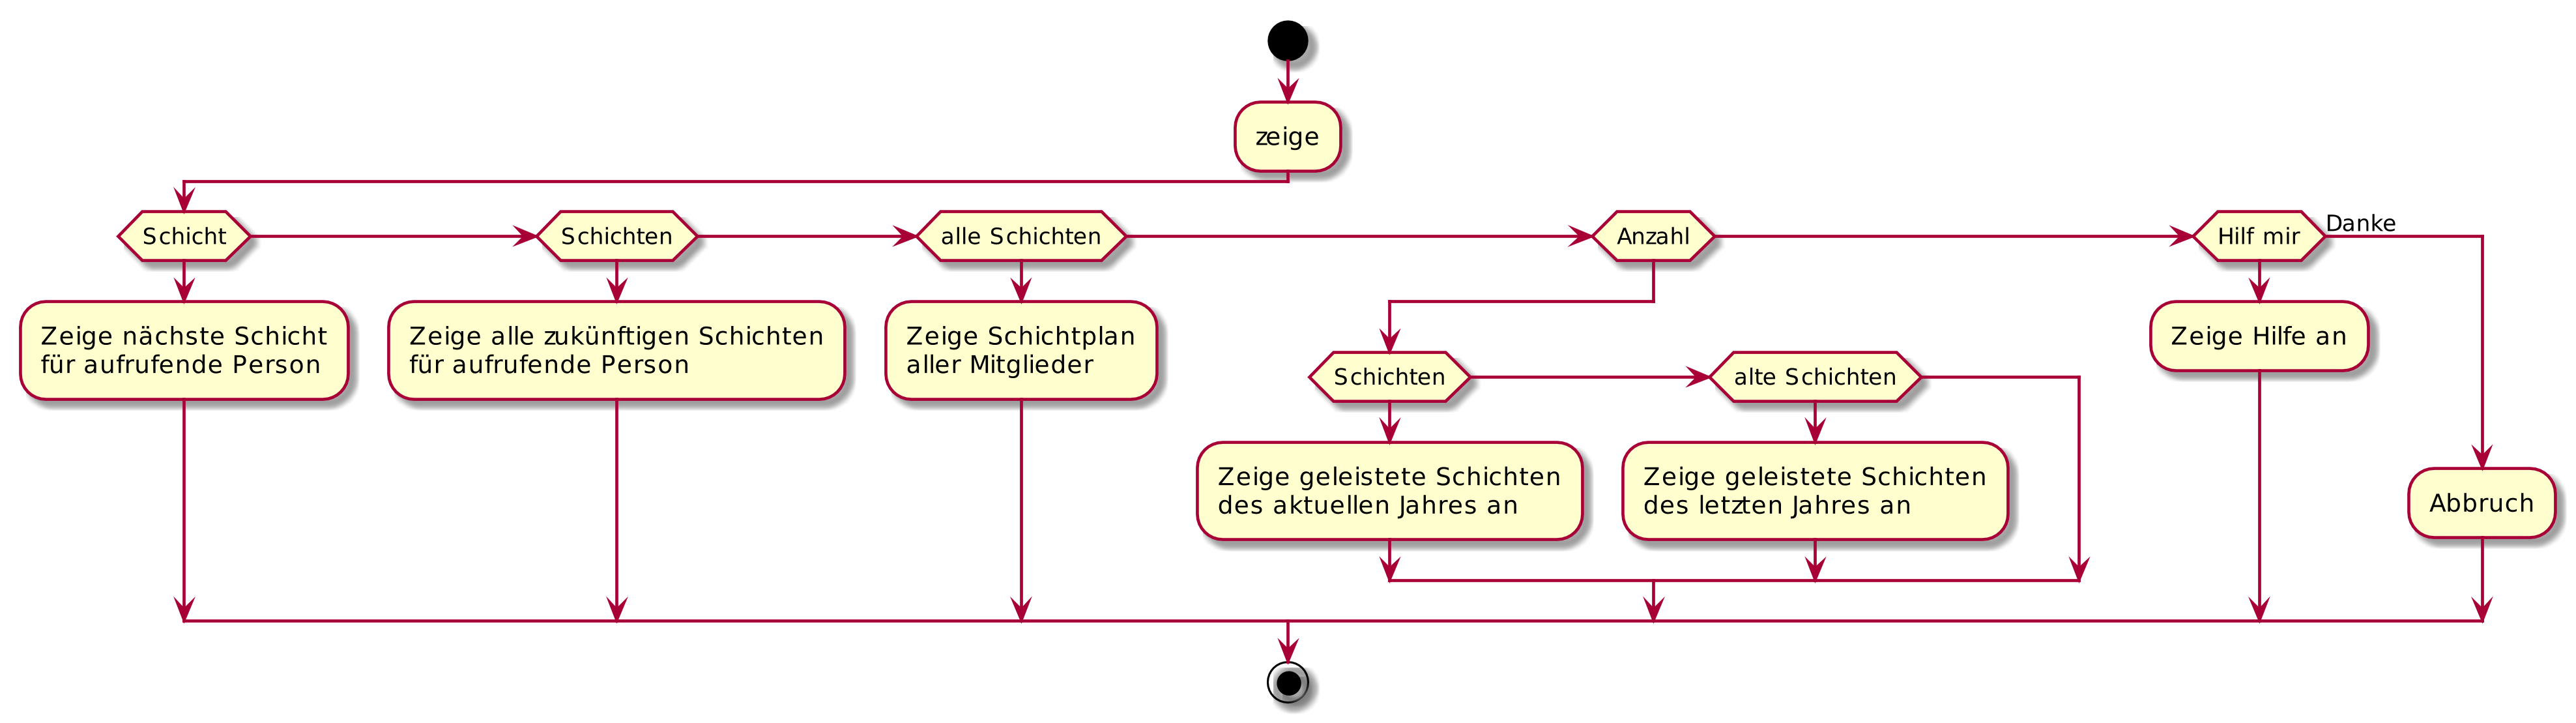
\includegraphics[width=\textwidth]{../docs/uml/activity-zeige.png}
    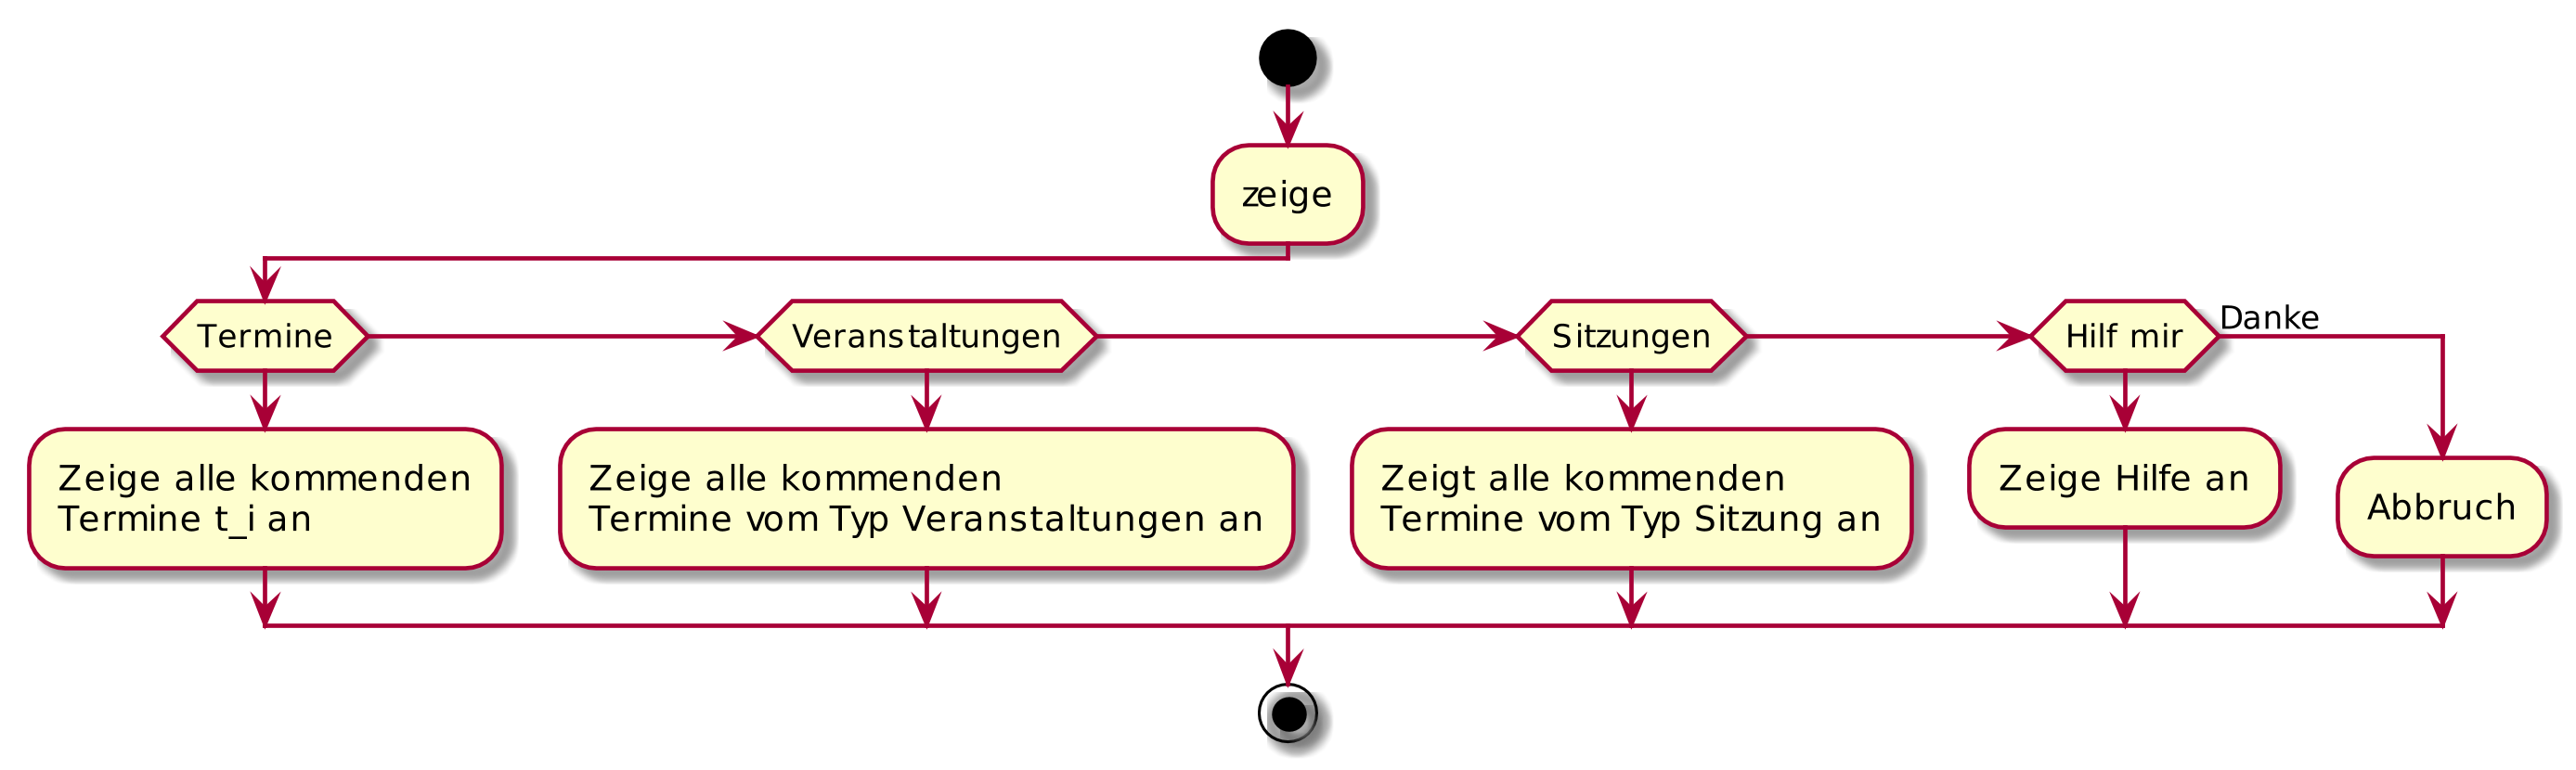
\includegraphics[width=0.9\textwidth]{../docs/uml/activity-zeige2.png}
    \caption{Aktivitätsdiagramme zum Anzeigen von Terminen}
    \label{img:activity-zeige}
\end{figure}

\begin{figure}[htbp]
    \centering
    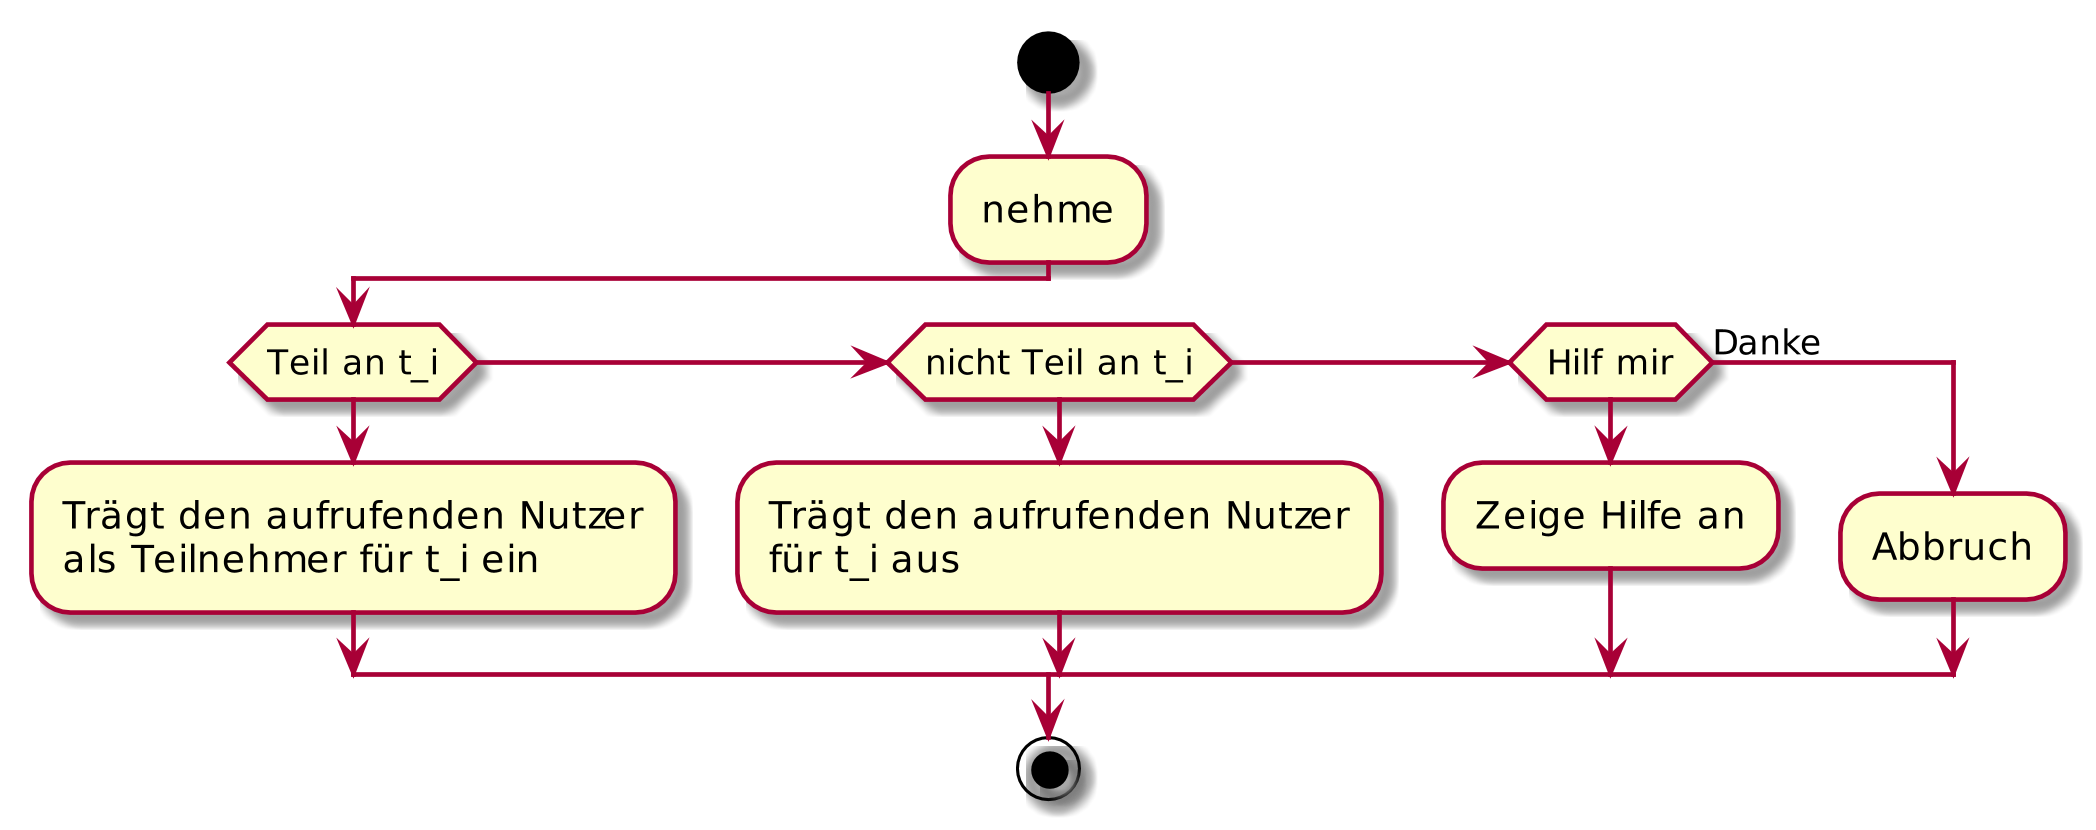
\includegraphics[width=0.7\textwidth]{../docs/uml/activity-teilnahme.png}
    \caption{Aktivitätsdiagramm zur Teilnahme an Terminen}
    \label{img:activity-teilnahme}
\end{figure}


Für die Befehle können auch Sätze gebildet werden, welche nachfolgend aufgeführt werden. Diese können kontextbezogen sein, sodass sich der Bot ähnlich wie ein natürlicher Gesprächspartner verhält. Ein Beispiel hierfür ist in \autoref{tab:satzinteraktion} zu sehen.

\begin{table}[H]
\centering
\begin{tabular}{|l|l|}
\hline
\textbf{Satz} & \textbf{Bedeutung }\\
 \hline
Wann ist die nächste Schicht? & zeigt die nächste Schicht an \\
\hline
Trag mich ein. & trägt den Aufrufer für die nächste Schicht ein \\
% \makecell{trägt den Aufrufer für den Termin ein, wenn nur eine\\ Schicht vorhanden ist / fragt nach, in welche Schicht\\ der Aufrufer eingetragen werden soll, wenn mehr als\\ eine Schicht vorhanden ist} \\
\hline
Danke & bricht die Konversation ab \\
\hline
\end{tabular}
\caption{kontextabhängige Befehle}
\label{tab:satzinteraktion}
\end{table}

Durch das Beispiel wird offensichtlich, dass der Bot den Kontext, in dem sich die Unterhaltung befindet, speichern muss. Dies ist pro Konversation und demnach pro Nutzer durchzuführen. Die Autoren gehen davon aus, dass eine Konversation nur einen Kontext besitzt. Es werden daher Konversationen ausgeschlossen, welche zwei Themen besitzen und diese sporadisch oder unvorhersehbar ändern.

Sollte der Satz \textit{Trag mich ein.} ohne Kontext geäußert werden, so soll keine Aktion durchgeführt werden. Da der Bot einer Konversation beiwohnen könnte, welche mit einem anderen Nutzer geführt wird, ist keine Aktion erforderlich oder gewünscht. Sollte der Bot jedoch zuvor den Satz \textit{Wann ist die nächste Schicht} aufgreifen, so soll er sich, wie eine natürliche Person, angesprochen fühlen und darauf reagieren. Weiterhin ist nun ein Kontext vorhanden, wodurch der nächste Satz eine Bedeutung erhält und nicht mehr ignoriert werden darf.

Das Wort \textit{Danke} dürfte auch sehr häufig in normalen Gruppendiskussionen geäußert werden, ohne dass der Bot dabei direkt angesprochen wird. Daher r ist es wichtig, auf dieses Wort nur im Kontext einer Konversation mit dem zu reagieren, da nur dort den Nutzern die kontextspezifische Bedeutung von Danke bewusst ist.

Aufgrund dessen entschieden sich die Autoren weitere Befehle einzuführen, welche den Bot natürlich wirken lassen sollen. Diese können in \autoref{tab:natuerlicheinteraktion} eingesehen werden. Weiterhin werden jene Sätze, auf die reagiert werden sollen, in der EBNF\footnote{Erweiterte Backus-Naur-Form} dargestellt.
% ACRONYM EBNF

\texttt{V = "Veranstaltungen"}\\
\texttt{T = "Termine"}\\
\texttt{S = "{}Sitzungen"}

\texttt{Frage1 = "Kann mir \{irgend\}jemand sagen"{} $|$ "Weiß \{irgend\}jemand"{} $|$\\ "Wer weiß"{} $|$ "Wieso sagt mir niemand"}\\
\texttt{Apell1 = "{}Sag\{e\} mir endlich"{} $|$ "Jetz\{t\} sag\{e\} schon"}\\
\texttt{Frage2 = "Wann haben wir die nächsten"{} $|$ "Wann sind die nächsten"}

\begin{table}[H]
\centering
\begin{tabularx}{\textwidth}{|p{5cm}|X|}
	\hline
	\textbf{Satz} & \textbf{Antwort} \\
	\hline
	\texttt{"Bob?"} & @\texttt{<Aufrufer>} Wie kann ich dir helfen? Mit \texttt{hilfe} zeige ich dir meine Hilfe. \\
	\hline
	{\texttt{Frage1 ", wann ich Bardienst habe?"{} $|$ Apell1 ", wann ich Bardienst habe"{} "."$|$"!"}} & @\texttt{<Aufrufer>} Dein nächster Bardienst ist am \texttt{<Datum>} von \texttt{<Beginn>} bis \texttt{<Ende>}.\\
	\hline
	\texttt{Frage2 "{} "{} V$|$S$|$T "?"} & @\texttt{<Aufrufer>} Die nächsten 5 \texttt{<V$|$S$|$T>} finden an folgenden Daten statt: \texttt{<Daten und Sichten>}\\
	\hline
	\texttt{"Wann finden die nächsten "{} V$|$S$|$T "{} statt?"} & Die nächsten 5 \texttt{<V$|$S$|$T>} finden an folgenden Daten statt: \texttt{<Daten und Sichten>}\\
	\hline
	\texttt{"Wird noch jemand für die nächste "{} V "{} gebraucht?"} &  Folgende Schichten benötigen noch Teilnehmer: \texttt{<Schicht>} \texttt{<Anzahl>} \\
	\hline
\end{tabularx}
\caption{natürliche Interaktion}
\label{tab:natuerlicheinteraktion}
\end{table}


\subsection{Datenbankauswahl}
\label{datenbankauswahl}
Für die Auswahl der Datenbank müssen ebenfalls die Anforderungen betrachtet werden. So muss die Datenbank eine Opensource-Lösung sein, jedoch nicht unter einer MIT-/BSD-ähnlichen Lizenz stehen, da diese nur benutzt und nicht verändert oder erweitert werden muss. Eine Opensource-Lösung ist für die Datenbank angebracht, da keine Lizenz- oder andere Kosten anfallen sollen. Weiterhin ist damit die Sicherheit gegeben, dass die Datenbank beliebig lange genutzt werden kann, da keine Lizenzen auslaufen können oder Updates erzwungen werden, welche die Funktionalität beeinflussen können. Die Sicherheit und Performance stehen an untergeordneter Stelle, da im Verein des Auftraggebers weniger als 100 Mitglieder erwartet werden, was die Effizienz der Datenbank in den Hintergrund rückt. Weiterhin werden durch ein Vertrauensverhältnis innerhalb des Vereins und dem regelmäßigen Wechsel der Rollen der Mitglieder keine Sicherheits- und Rechtebetrachtungen benötigt.

Grundsätzlich werden zwei verschiedene Ansätze für die Datenbank in Betracht gezogen. Es können relationale oder NoSQL-Datenbanken betrachtet werden. Der Einsatz von NoSQL wird durch folgende Kriterien begünstigt.

\begin{itemize}
	\item effizienter Umgang mit großen Datenmengen
	\item hohe Skalierbarkeit und Flexibilität
	\item hohe Redundanz
	\item häufige Änderungen der Datenstruktur
\end{itemize}
% https://www.tecchannel.de/a/datenbanksysteme-im-vergleich-mysql-vs-mongodb,2038219,5

MongoDB hat als NoSQL-Datenbank den zusätzlichen Vorteil, dass ein objektorientiertes Datenmodell verwendet werden kann, was einfache Abfragen mittels Programmiersprachen wie Javascript ermöglicht. Da die Abfragen jedoch in der Anzahl beschränkt sind, und damit kein großer Aufwand in der Implementierung stattfinden muss, können diese in eigens erstellte Funktionen implementiert werden. Dadurch, dass keine der genannten Kriterien auf die gegebenen Anforderungen zutrifft oder notwendig ist, entschieden sich die Autoren für eine SQL-Lösung.
%https://www.tecchannel.de/a/datenbanksysteme-im-vergleich-mysql-vs-mongodb,2038219,4

Laut der Popularitätsbewertung auf {dbranking} liegt MySQL als GNU-lizensierte Datenbank an erster Stelle. Die genutzten Kriterien sind für das Projekt ebenfalls Teilweise relevant. So sind die Bewertungskriterien für die Anzahl der Nennungen des Systems auf Websites, das allgemeine Interesse an dem System und die Häufigkeit von technischen Diskussionen über das System gute Indizien für die Zukunftssicherheit, Hilfe für optimale Nutzungsmöglichkeiten und die Fehlerbehandlung.
%https://db-engines.com/de/ranking
%2018-03-13



\subsection{Datenbankschema}

Das Datenbankschema soll laut Anforderung unabhängig von einem spezifischen Chatbot nutzbar sein. Falls ein Chatbot ausgetauscht oder andere Interaktionsmethoden hinzugefügt werden, darf die Datenbank entsprechend keine Abhängigkeiten besitzen. Es wird deshalb ein Datenbankschema angelegt, welches nur die Terminverwaltung abbildet und anschließend eine Erweiterung hinzugefügt, welche die notwendigen Schlüssel auf die verwendete Plattform abbildet.

Die Autoren haben die Struktur der derzeitigen manuellen Terminverwaltung erfasst und daraus ein Schema entworfen. 
Das im Verlauf des Entwurfsprozesses spezifizierte Datenbankschema basiert auf in diesem Kontext wichtigen Begriffen, welche im Folgenden näher erläutert werden.

Jeder Termin hat eine Bezeichnung, wie beispielsweise eine Weihnachtsfeier, Sitzung oder ein Afterwork. Diese Bezeichnungen werden Termintypen genannt und können mehr als einmal auftreten, wobei die Bezeichnungen nach deren Festlegung nicht direkt Terminen zugeordnet werden müssen. So kann eine Bezeichnung Weihnachtsfeier eingeführt werden, diese jedoch noch nicht geplant sein.

Weiterhin gibt es Zeitpunkte oder Zeitspannen, zu denen Termine stattfinden. Der Begriff Termin legt jedoch nicht fest, ob es sich um eine Zeitspanne oder einen Zeitpunkt handelt. So kann der Beginn einer Sitzung festgelegt werden, deren Ende jedoch nicht. Eine Andere Sicht auf Termine wäre die planmäßige Dauer eines Afterworks, wobei der Anfang und ein voraussichtliches Ende bekannt sind.

Wenn ein Termin festgelegt wird und dieser häufiger als einmal auftreten kann, ist es möglich, dass auch die Zeitspannen und Zeitpunkte mehr als einmal auftreten. Ein Afterwork beginnt laut den bekannten Informationen immer 19:00 Uhr, wobei zwei Schichten geplant sind, da die Mitglieder nicht über den ganzen Abend Bardienst haben wollen. Die erste Schicht dauert zwei Stunden, endet demnach gegen 21:00 Uhr, während die zweite Schicht 21:00 Uhr beginnt und meist bis 23:00 geht. Der Bardienst der letzten Schicht kann nach eigenem Ermessen festlegen, ob die Bar später schließt oder nicht. Für die Verwaltung ist letzteres jedoch nicht relevant.

Die Mitglieder sollen weiterhin die Möglichkeit haben, sich in diese Schichten einzutragen. Es muss deshalb eine Zuordnung der Schichten eines Termins und den Nutzern geben. 


Um die Anforderungen in einer Datenbank modellieren zu können, wurde ein Schema gemäß \autoref{img:db-schema} erstellt. Das Datenbankschema wurde gemäß der 3. Normalform (siehe \cite{CoddRelationalModelData1970}) erstellt. Dadurch ergeben sich Vorteile hinsichtlich Integrität und Datenzugriffszeit durch die Vermeidung redundanter Daten sowie der eindeutigen Zuordnung von Primärschlüsseln zu Tabellen (Konsistenz). Ein weiterer Vorteil der 3. Normalform ist die im Verhältnis zur 1. und 2. Normalform bessere Erweiterbarkeit, da alle Datensätze thematisch getrennt in jeweils eigenen Tabellen stehen (z.B. Trennung von Nutzer und SlackNutzer). 
Für den Einsatz als von weiteren Daten isolierter SlackBot wäre ein DB-Modell in 1. oder 2. Normalform aufgrund des einfacheren Aufbaus und weniger nötigen Lesezugriffen vorzuziehen. Dieses wurde aber hinsichtlich der gewünschten Integration in weitere Anwendungen in Form der 3. Normalform erstellt.
% \todo{das war ein 4-zeilen satz. kannst du den anders formulieren? ich will den nicht selbst kaputt machen}

Die strikte Aufteilung der Daten in den Tabellen bildet auch die Ebenen der verschieden Lebenszyklen der Datensätze ab, wobei hier zwischen langsam, mittel und schnell unterschieden werden konnte. Diese in \autoref{tab:db-speed} ersichtliche Unterscheidung basiert auf den relativen Unterschieden der Speicherfrequenz der Datensätze und ist daher nicht mit absoluten Werten zu bemessen. Beispielsweise ändern sich die Datensätze in der Tabelle NutzerSchicht erwartungsgemäß öfter als in der Tabelle SlackNutzer.

\begin{table}[H]
    \begin{tabularx}{0.9\columnwidth}{|l|X|X|}
    \hline
    \textbf{Datenspeicher} & \textbf{Beschreibung} & \textbf{Tabellen} \\
    \hline
    langsam & Daten werden selten geschrieben aber lange gespeichert & Nutzer, SlackNutzer, TerminTyp \\
    \hline
    mittel & Kombination schneller und langsamer Daten & Termin, Schicht \\
    \hline
    schnell & Daten werden oft geschrieben und relativ kurz gespeichert & NutzerSchicht, TerminSchicht \\
    \hline
    \end{tabularx}
    \caption{Vergleich der \enquote{Geschwindigkeiten} der Daten}
    \label{tab:db-speed}
\end{table}

Aktuelle Datenbankverwaltungssysteme wie MySQL, PostgreSQL und MariaDB bieten zum Beschleunigen der Lesezugriffe einen Query-Cache\footnote{siehe u.a. \url{https://dev.mysql.com/doc/refman/5.7/en/query-cache.html}}. Gemäß der hier vorgenommenen Unterteilung sind \enquote{schnelle} Daten besonders für den Cache-Einsatz geeignet, da auf diese am meisten Zugriffe erfolgen. 

Der Termintyp eines Termins wurde in eine extra Tabelle ausgelagert, da dieser mehrfach auftreten kann und deshalb redundant ist. Ein Termin muss eindeutig identifiziert werden können, weshalb eine ID eingeführt wird. Weiterhin erhält ein Termin ein Datum, welches den Tag des Beginns enthält. Ein Termintyp kann angelegt werden, ohne einem Termin zugeordnet zu sein, jedoch auch beliebig vielen Terminen zugeordnet werden, weshalb die Kardinalität \texttt{1 : 0..*} sein muss.

Schichten erhalten ebenfalls eine eigene Tabelle, da diese sonst redundante Informationen einführen würden. Um eine Schicht mit einem Termin zu verbinden, muss eine Zuordnung erfolgen, weshalb die Tabelle Terminschicht eingeführt wird. Über diese sind Termine, deren Namen und Schichten eindeutig identifizierbar. Es sollen Schichten angelegt werden können, ohne diese direkt Terminen bzw. der Terminschichttabelle zuweisen zu müssen, jedoch sollen Schichten beliebig vielen Terminen zugeordnet werden können. Die Kardinalität muss deshalb \texttt{1 : 0..*} zwischen Schicht und Terminschicht sein. Da ein Termin mehrere Schichten haben kann, demnach mehrfach in der Terminschichttabelle stehen kann und mindestens eine Zeit bzw. Schicht festgelegt haben muss, ist die Kardinalität zwischen Termin und Terminschicht \texttt{1 : 1..*}.

Nutzer erhalten ebenfalls eine eigene Tabelle mit einer ID. Die Nutzer müssen anschließend zu Terminschichten, d.h. zu eindeutigen Zeitspannen oder Zeitpunkten zugeordnet werden, wodurch eine Zuordnungstabelle Nutzerschicht benötigt wird. Da sich ein Nutzer in mehrere Schichten eintragen kann, jedoch auch keine Schicht belegt haben muss, ist die Kardinalität zwischen Nutzer und Nutzerschicht \texttt{1 : 0..*}. Eine Terminschicht muss keine Zuordnung zu einem Nutzer haben. Dies ist der Fall, wenn sich kein Nutzer für eine Schicht eintragen ließ. Die Kardinalität zwischen Terminschicht und Nutzerschicht ist dementsprechend ebenfalls \texttt{1 : 0..*}.

Die Zuordnung zu den verwendeten Chatplattformen ist nicht Teil der Terminverwaltung, soll jedoch nicht ausgelassen werden, weshalb eine Tabelle \texttt{<Plattform>}nutzer für jede Plattform angelegt werden kann, welche die IDs der Nutzer zu den Namen innerhalb jener zuordnet. Ein Nutzer einer Plattform ist hierbei immer eindeutig einem internen Nutzer zugeordnet. Ein interner Nutzer muss jedoch nicht Mitglied jeder Plattform sein. Es ist denkbar, dass sich ein Nutzer auf einer bestimmten Plattform mehr als einen Account anlegt und diesen mit dem intern eindeutigen Nutzer verbinden möchte. Dieser Fall soll nicht ausgeschlossen werden, weshalb die Kardinalität zwischen \texttt{<Plattform>}nutzer und Nutzer \texttt{0..* : 1} betragen muss.

Die Umsetzung der vorgestellten Informationen ist in \autoref{img:db-schema} ersichtlich.


% Hier das DB-Schmea rein und eine Fremdschlüsseltabelle für die Slack-Nutzernamen und bla

\begin{figure}[htbp]
    \centering
    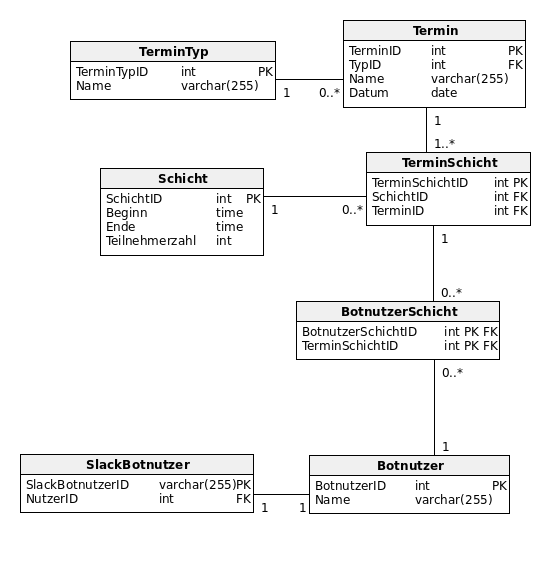
\includegraphics[width=\textwidth]{../docs/uml/Steckerbot-DB.png}
    \caption{Schema der Termin-Datenbank}
    \label{img:db-schema}
\end{figure}


\subsection{Kommunikationsschnittstellen}

Die Kommunikation zwischen der Datenbank und dem Chatbot erfolgt auf dem gleichen Host, weshalb keine besonderen Fälle beachtet werden müssen. Der Kommunikationspfad zwischen dem Chatbot und Slack wird jedoch über ein Hochschulnetzwerk durchgeführt. In diesem sind in das Netzwerk des Clubs nur die Ports 80 und 443 freigegeben. In der Standardkonfiguration bindet sich Hubot an Port 8080, der aber durch Setzen der Umgebungsvariable \texttt{PORT} geändert werden kann.

Eine erste Untersuchung des Netzwerkverkehrs zeigt jedoch weitere Ports, wie aus \autoref{img:packetports} zu entnehmen. Folgende Testumgebung kam hierbei zum Einsatz:
Die Standardkonfiguration Hubots wurde mittels docker-compose (Details siehe Abschnitt Containerisierung) lokal gestartet und der Netzwerkverkehr an der virtuellen Netzwerkbrücke mittels Wireshark aufgezeichnet. In der Standardkonfiguration greift der in NodeJS laufende Hubot auf den Redis-Container als \enquote{Brain} zu, was standardmäßig über Port 6379 erfolgt. Über Port 443 werden HTTPS-Verbindungen zum Slack-Server aufgebaut um beispielsweise Profilbilder nachzuladen.

Über die in diesem Beispiel genutzten Ports 43642 und 47230 erfolgt die weitere Kommunikation des Bots. Bei einem Neustart des Botclients ändern sich diese Ports, bleiben aber im Bereich der Non-Standard-Ports\footnote{Standardports unter \url{https://www.iana.org/assignments/service-names-port-numbers/service-names-port-numbers.xhtml}}. Für den Betrieb des Bots hinter einer Firewall mit Port-Whitelisting\footnote{alle Ports geschlossen, nur gewünschte Ports erlaubt} ist dies ein unerwünschtes Verhalten. Da die Einschränkung jedoch nur eingehende Verbindungen betrifft, war das Verhalten akzeptabel. Eine aus diesen Einschränkungen abgeleitete Systemarchitektur ist dem Deploymentdiagramm in \autoref{img:deployment} zu entnehmen.
In diesem ist neben den Komponenten wie Datenbankserver, Firewall und Chatbot auch eine Schnittstelle für einen Abruf der Termindaten per iCal o.ä. abgebildet, welche für eine spätere Implementierung vorgesehen ist.

\begin{figure}[H]
    \centering
    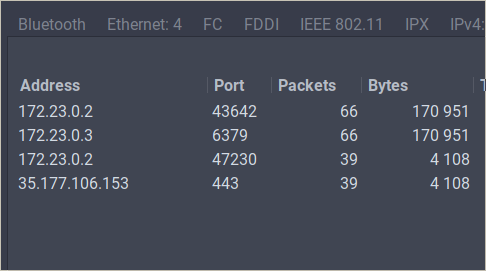
\includegraphics[width=0.7\textwidth]{img/packetports.png}
    \caption{Übersicht über von Hubot genutzte TCP-Ports}
    \label{img:packetports}
\end{figure}

%Ausgehend  doppeltes NAT aber Webseiten ok
\todo{NAT checken}

%Aus diesem Grund muss der Chatbot sich als Client mit Slack verbinden und darf keine Serveranwendung sein, welche ein Polling implementiert.

% vllt Grafik einfügen?
\begin{figure}[H]
    \centering
    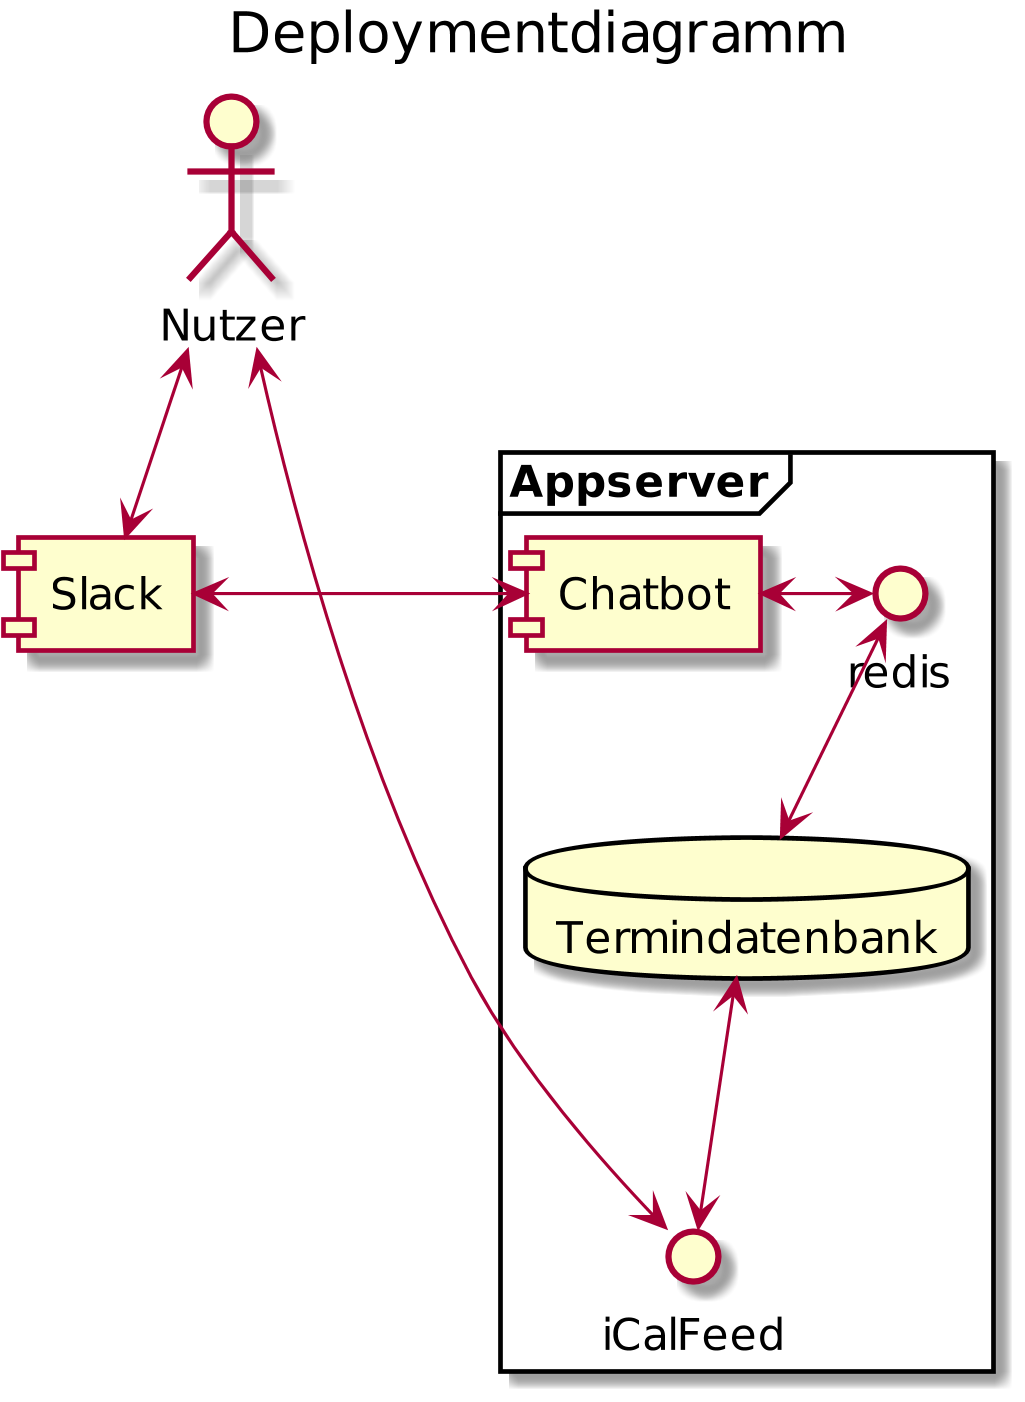
\includegraphics[width=0.5\textwidth]{../docs/uml/architecture.png}
    \caption{Deploymentdiagramm}
    \label{img:deployment}
\end{figure}


%Slack hat eine option globale UIDs zum bot durchzuleiten. nützlich, wenn mehrere Workspaces genutzt werden - ist das der fall? ferdi fragen.
% \todo{ERWEITERN + Slack-Workspace mit Ferdi klären}
